

%To run this example, follow the link

\subsubsection{Background}
In the field of quantum computing, researchers are continuously seeking efficient and robust methods to tackle complex problems. Adiabatic quantum computation (AQC) is one such approach, where a quantum system evolves gradually from an initial Hamiltonian to a final Hamiltonian that encodes the desired solution. According to the adiabatic theorem, if this evolution is slow enough, the system will remain in the ground state of the Hamiltonian throughout the process:

\begin{equation}
    H(t) = (1-\lambda(t))H_{\text{initial}} + \lambda(t)H_{\text{final}},
\end{equation}

where $\lambda(t)\in[0,1]$. However, implementing AQC in practical scenarios faces challenges arising from external noise, imperfections, and the need for long evolution times. To overcome these limitations and enhance the efficiency of adiabatic evolution, one promising approach to solve this problem is the Quantum Approximate Optimization Algorithm (QAOA), where a parameterized quantum circuit (ansatz) prepares a trial state to approximate solutions for optimization problems. By optimizing the ansatz parameters, QAOA seeks to find the optimal values that minimize or maximize the objective function, which encodes the problem's energy landscape.

However, practical implementations of QAOA face challenges due to noise, decoherence, and the complexity of parameter optimization. To enhance its performance and robustness, the Counterdiabatic Quantum Approximate Optimization Algorithm (CD-QAOA) introduced the counterdiabatic (CD) term:
\begin{equation}
    H_{\text{CD-QAOA}} = (1 - \lambda(t))H_{\text{initial}} + \lambda(t)H_{\text{final}} + H_{\text{CD}},
\end{equation}
It combines ideas from both AQC and the Quantum Approximate Optimization Algorithm (QAOA) by introducing one additional parameter per layer compared to QAOA. This results in shallower quantum circuits without compromising accuracy:
\begin{equation}
    U(\gamma, \beta)\to U(\gamma, \beta, \alpha), \quad F(\gamma, \beta)\to F(\gamma, \beta, \alpha),
\end{equation}
where $\alpha, \beta, \gamma$ represents the digitized parameters, $F$ is cost function and $U$ is evolution operator..
The CD term acts as an extra component in the Hamiltonian and is carefully designed based on the instantaneous eigenstates and eigenenergies of the evolving Hamiltonian.  The counterdiabatic term effectively suppresses errors and reduces the required evolution time, leading to enhanced efficiency and reliability in quantum computations.

To derive the precise form of the counterdiabatic term, various techniques, such as Lewis-Riesenfeld invariants and transitionless quantum driving, have been applied. The implementation of the CD term is tailored to the specific problem and dynamics of the quantum system, utilizing available control techniques. In cases where obtaining exact CD terms becomes challenging, an approximate CD driving approach is proposed, utilizing the nested commutator method\cite{Chandarana_2023} with the adiabatic gauge potential:

\begin{equation}
    A_{\lambda}^{(l)} = i\sum_{k=1}^{l}\alpha_{k}(t)[H_{a},[H_{a},...[H_{a}, \partial_{\lambda}H_{a}]]].
\end{equation}

DC-QAOA holds promise for solving a wide range of optimization problems, from combinatorial optimization to machine learning tasks and financial portfolio optimization. As quantum computing technology continues to advance, DC-QAOA represents an exciting avenue for leveraging the counterdiabatic term and parameter space digitization to unlock new frontiers in quantum optimization.

\textbf{Target problem}
\begin{itemize}
    \item[1.] Learn how to find the ground state of problem Hamiltonian
    \item[2.] Utilize quantum circuits to find optimized parameters
\end{itemize}
\textbf{Required Mindquantum functionalities}
\begin{itemize}
    \item[1.] gradient-based optimizer
    \item[2.] Batch quantum circuit simulator

\end{itemize}

\subsubsection{Implement}
As a mature application of QAOA, this algorithm requires two steps, which is building the ansatz circuit and optimization. Now let's look at how to implement Digitized-counterdiabatic quantum approximate optimization algorithm (DC-QAOA) into Ising spin model, the model is depicted in Fig.~\ref{fig:ising}. The initial state is choose as $H_{initial} = \sum_{i}\sigma_{i}^{x}$. The general form of the Hamiltonian of the 1D Ising spin model is given by
\begin{figure}
    \centering
    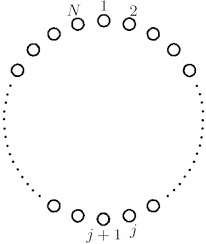
\includegraphics[width=0.5\linewidth]{5.4.1_figure/ising.jpg}
    \caption{Schematic picture of the Ising model}
    \label{fig:ising}
\end{figure}

\begin{equation}
    H_{final} = -\sum_{\langle i,j \rangle}J_{ij}\sigma_{i}^{z}\sigma_{j}^{z} - \sum_{i}h_{i}\sigma_{i}^{z} - \sum_{i}k_{i}\sigma_{i}^{x}.
\end{equation}
\begin{lstlisting}
# generate H_{initial} as H_{mixer}
# n_qubits is the number of qubits
def generate_h_mixer(n_qubits:int):
    h_mixer = QubitOperator()
    for i in range(n_qubits):
        h_mixer += QubitOperator(f'X{i}')
    return h_mixer
    
# generate H_{final} as H_{prob}
def generate_h_prob(n_qubits:int, J:float, h:float, k:float):
    h_prob = QubitOperator()
    for i in range(n_qubits):
        j = (i+1)%n_qubits
        h_prob += QubitOperator(f'Z{i} Z{j}', J)
        h_prob -= QubitOperator(f'Z{i}', h)
        h_prob -= QubitOperator(f'X{i}', k)
    return h_prob
\end{lstlisting}

In our case,  a pool of CD operators is defined using the nested commutator approach of the adiabatic gauge potential \cite{PhysRevResearch.4.013141}
$$A = \{\sigma^{y},\sigma^{z}\sigma^{y}, \sigma^{y}\sigma^{z}, \sigma^{x}\sigma^{y}, \sigma^{y}\sigma^{x} \}.$$

Here we present a 12 qubits system and we consider second-order $A = \sum_{i}\sigma_{i}^{z}\sigma_{i+1}^{y}$. For simplify, we choice  $J = -1, h = 0, k = -1$. Following we build an ansatz layer for DC-QAOA.
\begin{lstlisting}
def generate_h_cd(n_qubits:int):
    h_cd = QubitOperator()
    for i in range(n_qubits-1):
        h_cd += QubitOperator(f'Z{i} Y{i+1}')
    return h_cd
\end{lstlisting}

\begin{lstlisting}
n_qubits = 12
J, h, k = -1, 0, -1

h_prob = generate_h_prob(n_qubits, J, h, k)
h_mixer = generate_h_mixer(n_qubits)
h_cd = generate_h_cd(n_qubits)
\end{lstlisting}

In order to prepare the eigenstate for $H_{initial}$, we first put ${\rm prep\_circ}$, and then apply evolution operator on it.
\begin{lstlisting}
# generate the eigenstate for $H_{mixer}$
prep_circ = UN(H, n_qubits)

# choose two layer 
p = 3
ansatz_template = u_p + u_m + u_cd

ansatz = Circuit() + prep_circ
for i in range(p):
    ansatz += add_suffix(ansatz_template, str(i)) + BarrierGate()
\end{lstlisting}

As long as we have set up the ansatz circuit, we can change the number of layers or type of optimizer in order to find the optimal parameter set. We define cost function using
\begin{equation}
    E = \left<\psi_0\right|U^{\dagger}\ H_{prob} U\left|\psi_0\right>,
\end{equation}
where $U = \Pi_{i=0}^3 U_{cd}(\alpha_i)U_m(\beta_i)U_p(\gamma_i)$ and this is just the evolution operator.
\begin{lstlisting}
energys = []
# define cost function
def fun(x0, grad_ops, energys):
    f, g = grad_ops(np.array(x0))
    f = np.real(f[0, 0])
    g = np.real(g[0, 0])
    energys.append(f)
    if len(energys)%5==0:
        print(f"step: {len(energys)}, energy: {f}")
    return f, g
\end{lstlisting}

In this tutorial, we will optimize the gradient using BFGS optimizer\cite{chandarana2022meta}, which will have good enough results. If you plot the figure of mean energy, you will have result like Fig.~\ref{fig:dc}. Here, the green line is the exact eigenvalue of $H_{prob}$, the blue line is the mean value during the optimizing process, the orange line is QAOA with three layers. We can notice that DC-QAOA  has converged to the exact value in 70 steps within 0.5s. Comparing these two algorithm from the ability of estimating the ground state, DC has advantage over QAOA.
\begin{figure}
    \centering
    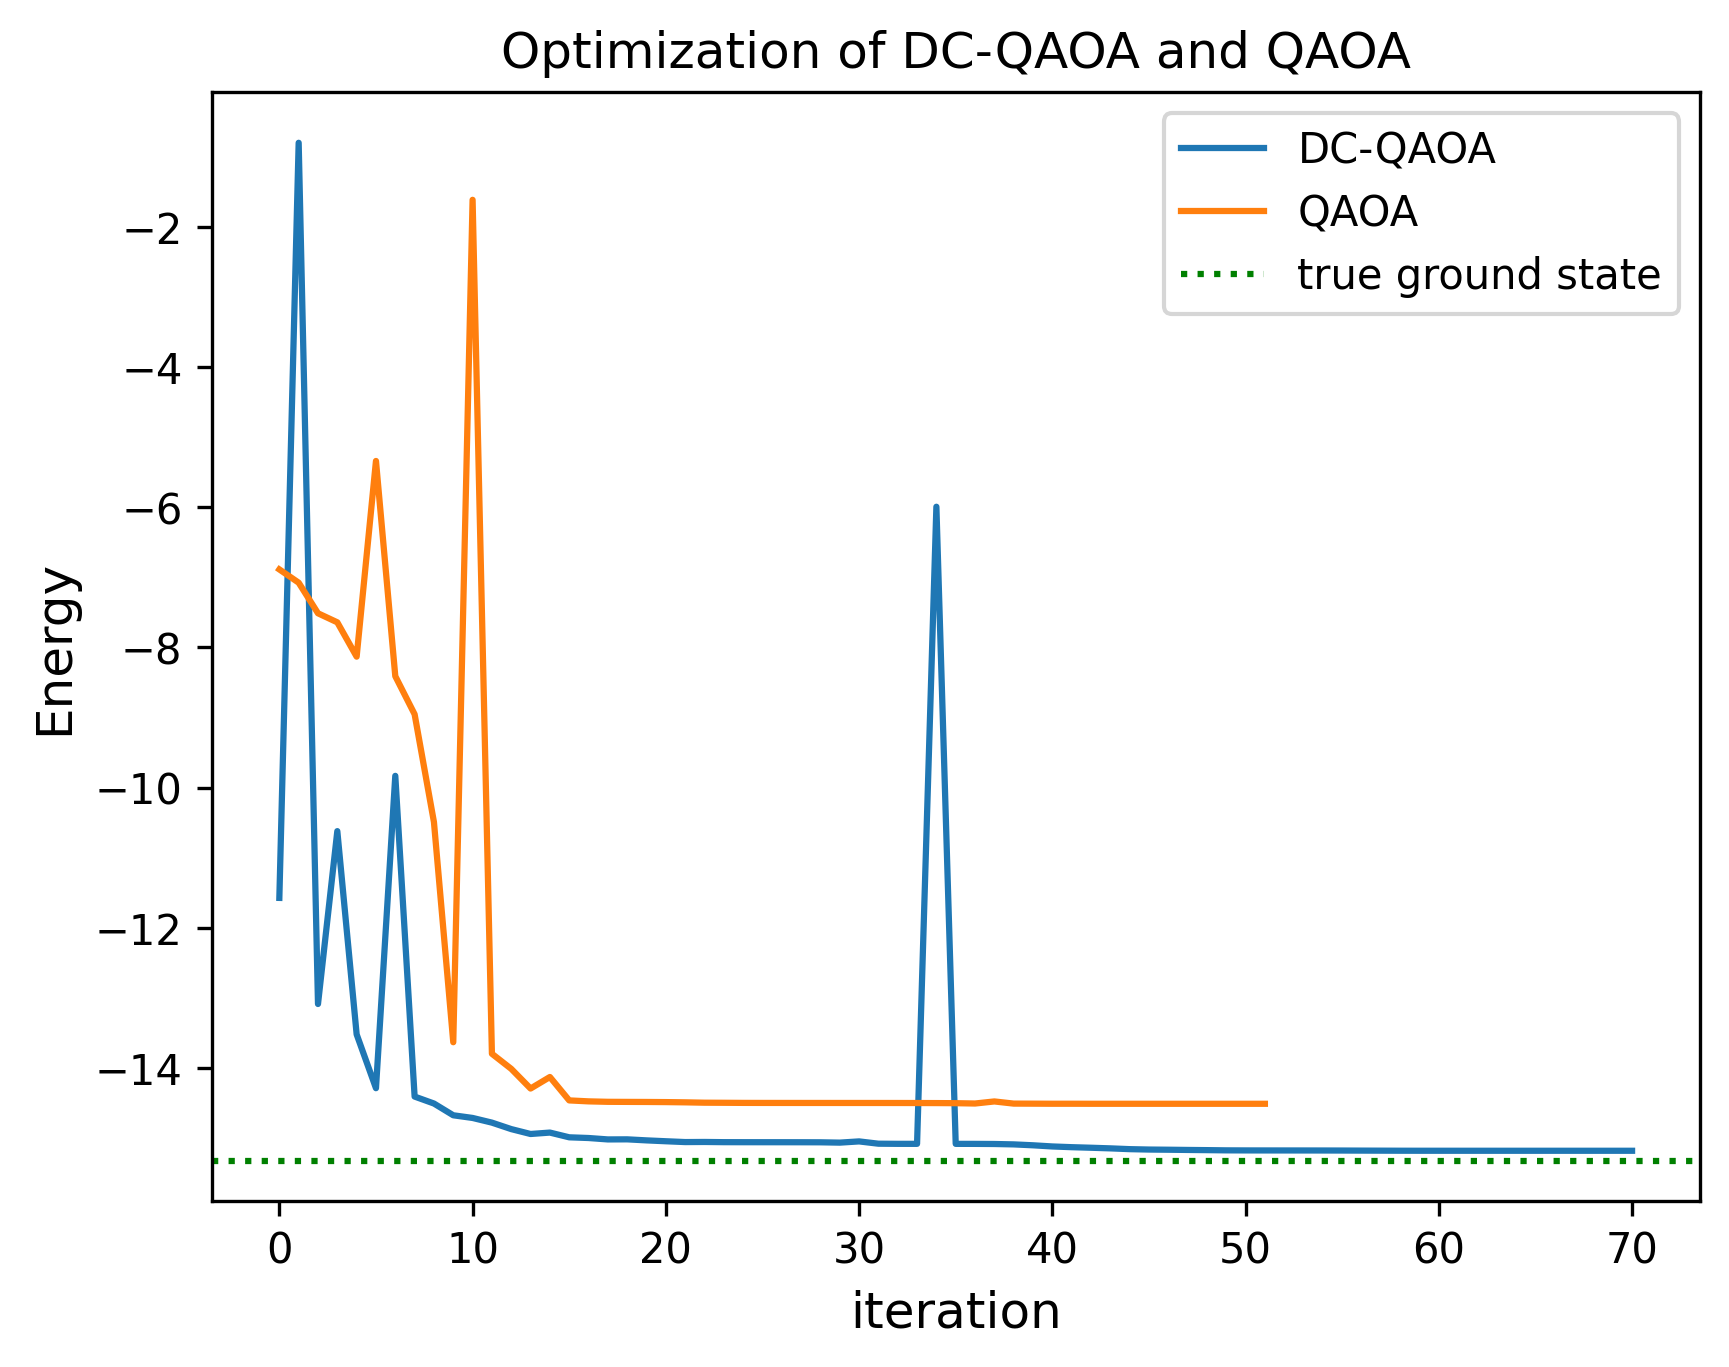
\includegraphics[width = 1 \linewidth]{5.4.1_figure/DC-WHITE.png}
    \caption{Mean Energy vs. iteration time}
    \label{fig:dc}
\end{figure}



